\documentclass[11pt,border=2pt]{standalone}
\usepackage{amsmath,amssymb}
\usepackage{xcolor}
\usepackage{tikz}
\usepackage{pgfplots}
\pgfplotsset{compat=1.18}
\usetikzlibrary{calc,arrows,positioning,fit,backgrounds,decorations.pathreplacing,patterns}
\definecolor{cElem}{RGB}{40,80,140}
\definecolor{cTrg}{RGB}{190,40,40}
\definecolor{cCell}{RGB}{225,238,248}
\definecolor{cAcc}{RGB}{240,200,120}
\definecolor{cGrey}{RGB}{120,120,120}
\definecolor{cVec}{RGB}{110,55,150}
\begin{document}
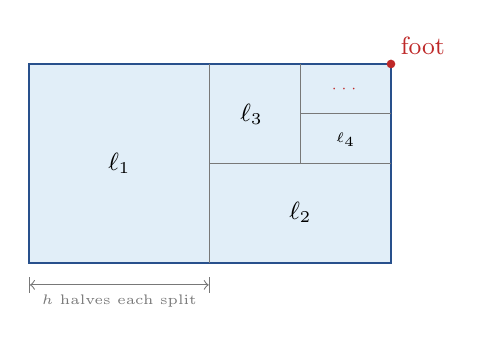
\begin{tikzpicture}[scale=4.6,font=\small]
  \fill[cCell] (0,0) rectangle (1,0.55);
  \draw[cElem,thick] (0,0) rectangle (1,0.55);
  % bisections marching toward the foot at (1,0.55)
  \draw[cGrey] (0.5,0) -- (0.5,0.55);
  \draw[cGrey] (0.5,0.275) -- (1,0.275);
  \draw[cGrey] (0.75,0.275) -- (0.75,0.55);
  \draw[cGrey] (0.75,0.4125) -- (1,0.4125);
  \fill[cTrg] (1,0.55) circle (0.012);
  \node[cTrg,above right=0pt,font=\small] at (1,0.55) {foot};
  \node at (0.25,0.275) {$\ell_1$};
  \node at (0.75,0.14)  {$\ell_2$};
  \node at (0.615,0.41) {$\ell_3$};
  \node at (0.875,0.34) {\tiny $\ell_4$};
  \node[cTrg,font=\tiny] at (0.875,0.48) {$\cdots$};
  \draw[|<->|,cGrey] (0,-0.06) -- (0.5,-0.06) node[midway,below,font=\tiny] {$h$ halves each split};
\end{tikzpicture}
\end{document}
